\documentclass{article}
\usepackage{fullpage}
\usepackage{indentfirst}
\usepackage{amsmath}
\usepackage{amsfonts}
\usepackage{array}
\usepackage{tipa}
\usepackage{tikz}
\usepackage{tikz-qtree}
\usetikzlibrary{matrix, arrows, automata}
\usepackage{natbib}
\usepackage{gb4e}
\noautomath
\newcommand{\Y}{$\checkmark$}
\newcommand{\R}{$\Rightarrow$}
\newcommand\myeq{\mathrel{\stackrel{\makebox[0pt]{\mbox{\normalfont\tiny def}}}{=}}}
\newcommand{\ap}{\approx}
\title{Register Dissimilation in Luoyang}
\author{Chris Oakden}
\begin{document}
\maketitle
\citet{Bao1990}, citing \citet{He1984}, provides evidence of register dissimilation from Luoyang, a Mandarin dialect. When a high-registered falling tone precedes another high-registered tone, it surfaces with low register. For example, two adjacent high-falling tones /53.53/ surface as a low-falling and high-falling tone [31.53]: 
\begin{center}
\begin{tabular}[t]{lll}
\textipa{iaN} & ma & `raise horses' \\
53 & 53 & base form \\
31 & 53 & sandhi form\\
\end{tabular}
\hspace{1cm}
\begin{tabular}[t]{lll}
\textipa{lO} & mi & `old rice' \\
53 & 53 & base form \\
31 & 53 & sandhi form\\
\end{tabular}
\end{center}
The phonetic forms [53] and [31] correspond to the tonal geometric configurations (+u;hl) and (-u;hl) respectively. Representation of the above examples in Bao's formalism is thus:
\begin{center}
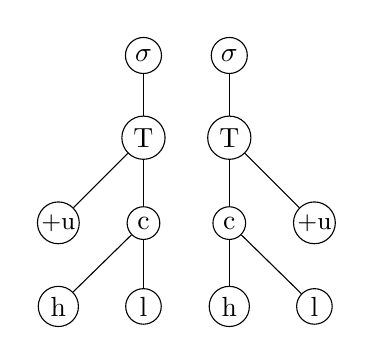
\begin{tikzpicture} [baseline = (y1.base)]
\matrix (m) [matrix of nodes, column sep = 1.5em, row sep = 1.5em]{
& \node[draw,circle, inner sep =2pt](x1){$\sigma$};  &  \node[draw,circle, inner sep =2pt](x2){$\sigma$};  \\
& \node[draw,circle, inner sep =2pt](y1){T}; &   \node[draw,circle, inner sep =2pt](y2){T}; \\
\node[draw,circle, inner sep =.5pt](z1){\small +u}; & \node[draw,circle, inner sep =2pt](z2){c}; &   \node[draw,circle, inner sep =2pt](z3){c}; & \node[draw,circle, inner sep =.5pt](z4){\small +u}; \\
\node[draw,circle, inner sep =2pt](t1){h}; & \node[draw,circle, inner sep =2pt](t2){l}; &  \node[draw,circle, inner sep =2pt](t3){h}; & \node[draw,circle, inner sep =2pt](t4){l}; \\
};
\draw (x1) -- (y1);
\draw (x2) -- (y2);
\draw (z1) -- (y1);
\draw (z2) -- (y1);
\draw (z2) -- (t1);
\draw (z2) -- (t2);
\draw (y2) -- (z3);
\draw (y2) -- (z4);
\draw (z3) -- (t3);
\draw (t4) -- (z3);
\end{tikzpicture}
\hspace{.3cm}
$\rightarrow$
\hspace{.3cm}
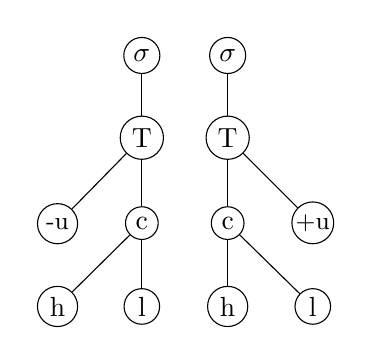
\begin{tikzpicture} [baseline = (y1.base)]
\matrix (m) [matrix of nodes, column sep = 1.5em, row sep = 1.5em]{
& \node[draw,circle, inner sep =2pt](x1){$\sigma$};  &  \node[draw,circle, inner sep =2pt](x2){$\sigma$};  \\
& \node[draw,circle, inner sep =2pt](y1){T}; &   \node[draw,circle, inner sep =2pt](y2){T}; \\
\node[draw,circle, inner sep =2pt](z1){\small -u}; & \node[draw,circle, inner sep =2pt](z2){c}; &   \node[draw,circle, inner sep =2pt](z3){c}; & \node[draw,circle, inner sep =.5pt](z4){\small +u}; \\
\node[draw,circle, inner sep =2pt](t1){h}; & \node[draw,circle, inner sep =2pt](t2){l}; &  \node[draw,circle, inner sep =2pt](t3){h}; & \node[draw,circle, inner sep =2pt](t4){l}; \\
};
\draw (x1) -- (y1);
\draw (x2) -- (y2);
\draw (z1) -- (y1);
\draw (z2) -- (y1);
\draw (z2) -- (t1);
\draw (z2) -- (t2);
\draw (y2) -- (z3);
\draw (y2) -- (z4);
\draw (z3) -- (t3);
\draw (t4) -- (z3);
\end{tikzpicture}
\end{center}
\citet{Bao1990} categorizes dissimilation as a feature-changing operation (non-elementary in Sagey's terms (cite)), a composite of deletion and insertion. We represent the process as in input-to-output mapping; the transduction is defined over one copy set.
\begin{equation}
\begin{aligned}
P^{\tau}_{\sigma}(x)&\myeq P_{\sigma}(x) & P^{\tau}_{T}(x)&\myeq P_{T}(x) & P^{\tau}_{c}(x)&\myeq P_{c}(x) \\
P^{\tau}_{+u}(x)&\myeq P_{+u}(x) \land final(x) & P^{\tau}_{-u}(x)&\myeq P_{+u}(x) \land \neg final(x) \\
P^{\tau}_{h}(x)&\myeq P_{h}(x) & P^{\tau}_{l}(x)&\myeq P_{l}(x) \\
\alpha^{\tau}(x)\ap y &\myeq\alpha(x)\ap y & \delta^{\tau}(x)\ap y &\myeq\delta(x)\ap y & succ^{\tau}(x)\ap y &\myeq succ(x)\ap y \\
\end{aligned}
\end{equation}
The transduction is straight-forward; in our terms, feature changing is redefining unary functions over register features. All other relations (including association, dominance, and linear order) are preserved from the input signature. 
\bibliographystyle{apalike}
\bibliography{references}
\end{document}